Roughly speaking, when working with multiple omics data, the integration phase requires that the data used for this step are ''connected'' between different omics.

%For example, if we want to investigate the epigenetic marks involved in the regulation of the gene expression of a particular disease, we need to collect data from \gls{chipseq} and \gls{rnaseq} experiments under the same experimental conditions.
%To do that, we need to collect as many samples as possible for each omics (because as higher is the number of samples as higher will be the power for estimating good results) to evaluate a certain number of variables/features (i.e. gene expression, methylation, \gls{tf}, etc.) for each sample.

%Moreover, when investigating multiple conditions, we need multiple replicates for each condition, in order to be able to well estimate and remove biases affecting the experiment and distinguish technical or biological variability as well as other sources of variation.
%(Biostatisticians typically say that the number of replicates must never be lower than 3, indeed some statistical methods cannot work properly with a number of replicates lower than this.)

%To summarize, when working with multi-omics data, we need to collect samples of the interested cellular line for the disease/condition we want to study.
%Moreover, to understand multiple mechanisms affected by the disease we need to collect multiple omics for each biological aspect (i.e. \gls{chipseq} and \gls{rnaseq}).
%Additionally, for each omics, we need to collect multiple samples for each condition (i.e. healthy and tumor).
%Therefore, typically multi-omics datasets consist in a bunch of short reads files (each of them corresponding to a specific sample in specific conditions). 

After some preprocessing (alignment, quantification, etc.) the results are combined in specific omics matrices $X_k$ with  $k=1,...,m$, where \textit{m} denotes the number of omics, such that $dim[X_k]=[n_k, p_k]$, where $n_k$ is the number of samples (such as patients, tissues, etc.) and $p_k$ the number of observed variables (features) on the specific omics.
In particular, for each of the \textit{m} matrices it is possible to investigate different biological questions, depending on the nature and availability of the data.
We can distinguish between the variable based analysis, where each matrix has the same varibles and differs on the samples, and the samples based analysis, where for the same samples across multiple omics we have different features.
In the first case we can answer relevant common biological questions on the features (such as genes, genomic regions, etc.) across multiple omics, while in the second case we can answer biological questions related to the samples observing different variables at each omics level.

Once we collected all the required samples, we can either start analyzing each omics individually and/or integrating them to better understand the cellular behaviours involved in the studied disease.
Depending on the number of collected samples, we can choose from different methodologies to apply.
If we have few numbers of samples, we can decide to work on single omics analysis and then to integrate the results.
Otherwise, when having a high number of samples we can use deeper statistical methodologies, such as network fusion techniques for constructing multiple levels regulatory networks \cite{Angelini2014c, Rohart2017, Argelaguet2018}.

In order to account for these kind of studies, inside \gls{igro} we are implementing several aspects and interfaces to help and guide the user to achieve integrated results.

\subsection{The main interface}
\gls{igro} is a web platform fully developed in R with aid of Shiny libraries, combining the power of the R statistical instrument with HTML5/javascript flexibility.

Shiny apps are typically designed for small applications, allowing a very easy and versatile way for developing and releasing them.
The basic structure of a shiny app is based on two main entities, the \gls{sui} and the \gls{ss}.
The first one includes all the aesthetic components which the user interacts with, while the \gls{ss} processes all the computations.

Natively, shiny apps support only one server, but when the needs grow up and multiple interfaces are needed the things become more complicated. 

Our case is composed of a high number of methodologies for multiple-omics problem solving and required a more complex implementation.
To account our problematic, we choose to build \gls{igro} as self-containing modules, by using recently born shiny modules technology\footnote{\url{https://shiny.rstudio.com/articles/modules.html}}.
In such a way, the main shiny app can be shredded into multiple "mini apps", each one with its own \gls{sui} and \gls{ss}.
This approach is totally invisible to the final user, but helps the developer for the maintainability and the extensibility of the entire tool.
Indeed, when future needs arise for the implementation of novel functionalities, it is necessary just to implement a novel module.

Our tool presents itself with an upper menu of main topics organized by main scopes. 
For each of these topics, a sub-menu with specific functionalities is available.
When additional functionalities are available, they appear in a left side menu.
In order to well set up the parameters for each functionality, an additional side menu is presented with the parameters and their possible values for the right setup (figure \ref{fig:integrhomain} shows a general representation of the main interface).

\begin{figure}[ht]
\centering
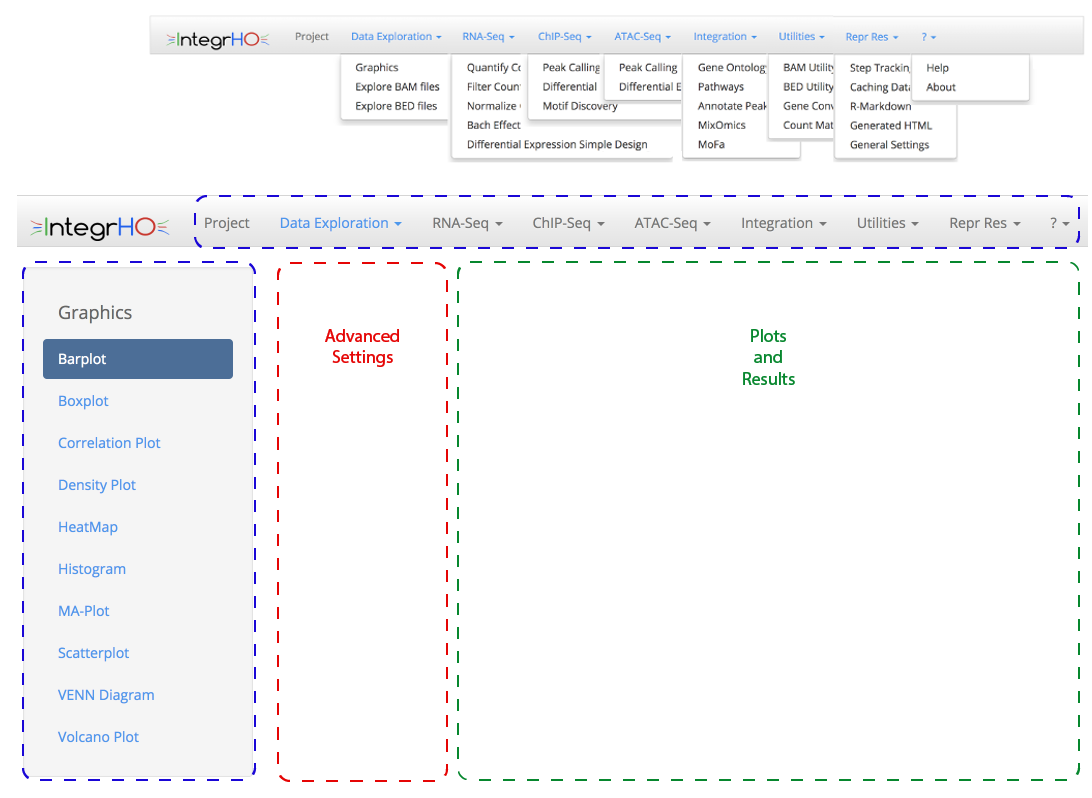
\includegraphics[width=\textwidth, keepaspectratio]{img/integrho/interface.png}
\caption[\gls{igro} main interface]{\gls{igro} main interface description. A main menu in the upper part is presented with all the available main functionalities, and a left side menu is presented with additional functionalities (in blue). Red part indicates the settings for each functionality within the parameter setup. While in green results in table or graphical form are presented.}
\label{fig:integrhomain}
\end{figure}

Once the user set up the required parameters and pressed the section button, the parameters are processed and the results are shown in graphical or table format in the main part of the interface.

We decided to implement \gls{igro} as a design file based software.
Because of the high number of samples needed for the data analysis, the user needs to specify several variables describing each sample.
This is useful for defining samples belonging to the same condition, and to specify which is the omics for each sample, and some additional describing variables.
The design file information will be used during all the following steps of the analysis.

Before to proceed to the data analysis, it is mandatory for the user to set up the project with a dedicated interface.
The user has to upload the design file which describes the information related to its samples.
Some of them are mandatory, such as the filename (with path) of the \gls{bam} files and the conditions of each sample, while others are optional as the tissue or the run id. 
It is also possible to manually edit the design file directly from the interface (figure \ref{fig:integrhodesign}).

The choice of using a mandatory variable describing the path of  \gls{bam} filenames is due to a \textit{Shiny} library limitation. 
Because of its ''UI-server'' structure, shiny applications, when using a \lstinline!fileInput! widget, make a temporary copy of the selected file(s).
But this aspect becomes really problematic when a file can reach several gigabytes of memory on disk, as one or more \gls{bam} files can.
Even if there are alternative packages, such as \textit{shinyFiles} \cite{Pedersen}, offering the possibility to solve the problem, they are not very well tested over multiple platform architectures, bringing us to choose for this workaround solution.

\begin{figure}[ht]
\centering
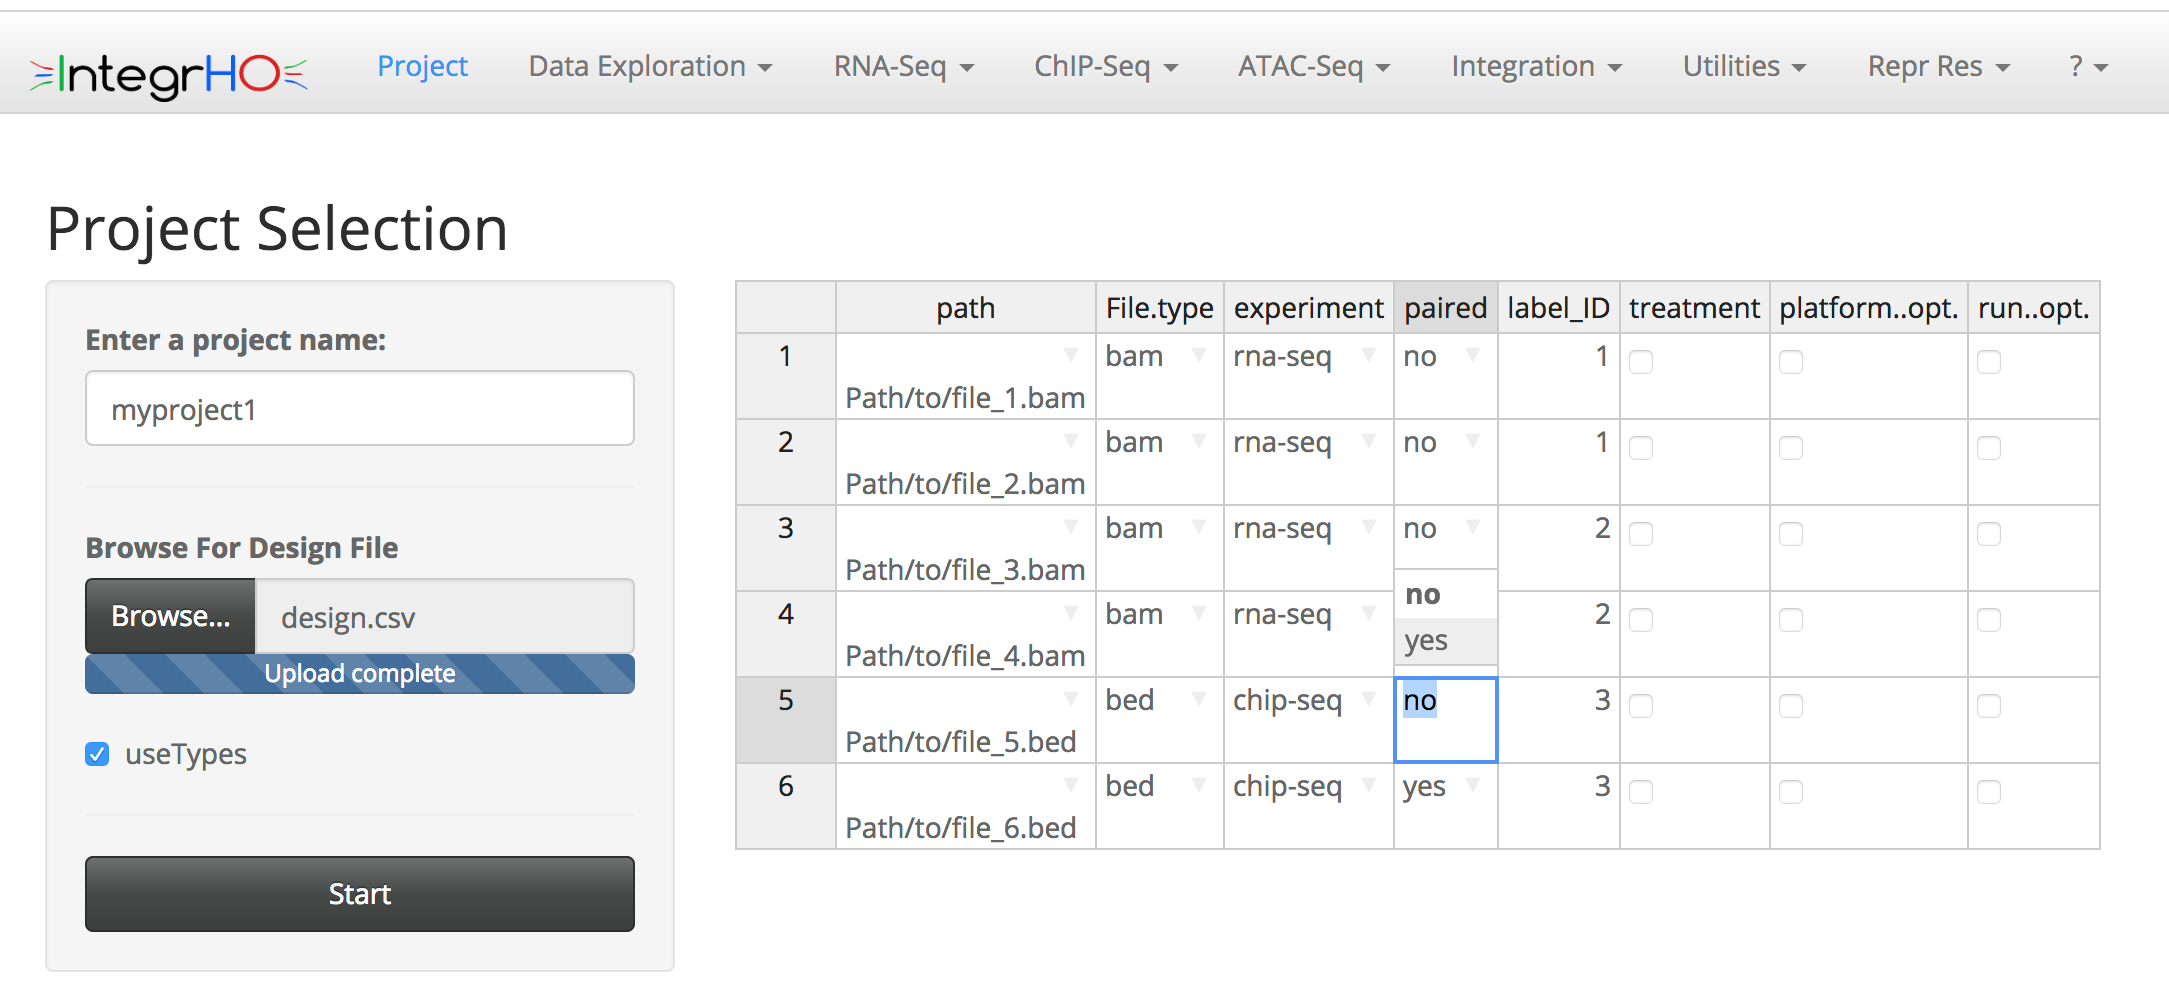
\includegraphics[width=\textwidth, keepaspectratio]{img/integrho/design.png}
\caption[\gls{igro} design interface]{The project design \gls{igro} interface. The user has to insert a name for the project and to load a design file.
The design file can be edited through the interface itself.}
\label{fig:integrhodesign}
\end{figure}

Using the project interface, \gls{igro} creates inside the working directory (returned by the \lstinline!getwd()! function) a dedicated folder with all the required sub-folders and stores all the basic information of the project into an ad-hoc designed \lstinline!R6ProjectClass!, which is re-used during the whole session to speed up the configuration of each step of the analysis (Figure \ref{fig:integrhotree} shows a representation of a typical folder tree produced for a project).

\begin{figure}[ht]
\centering
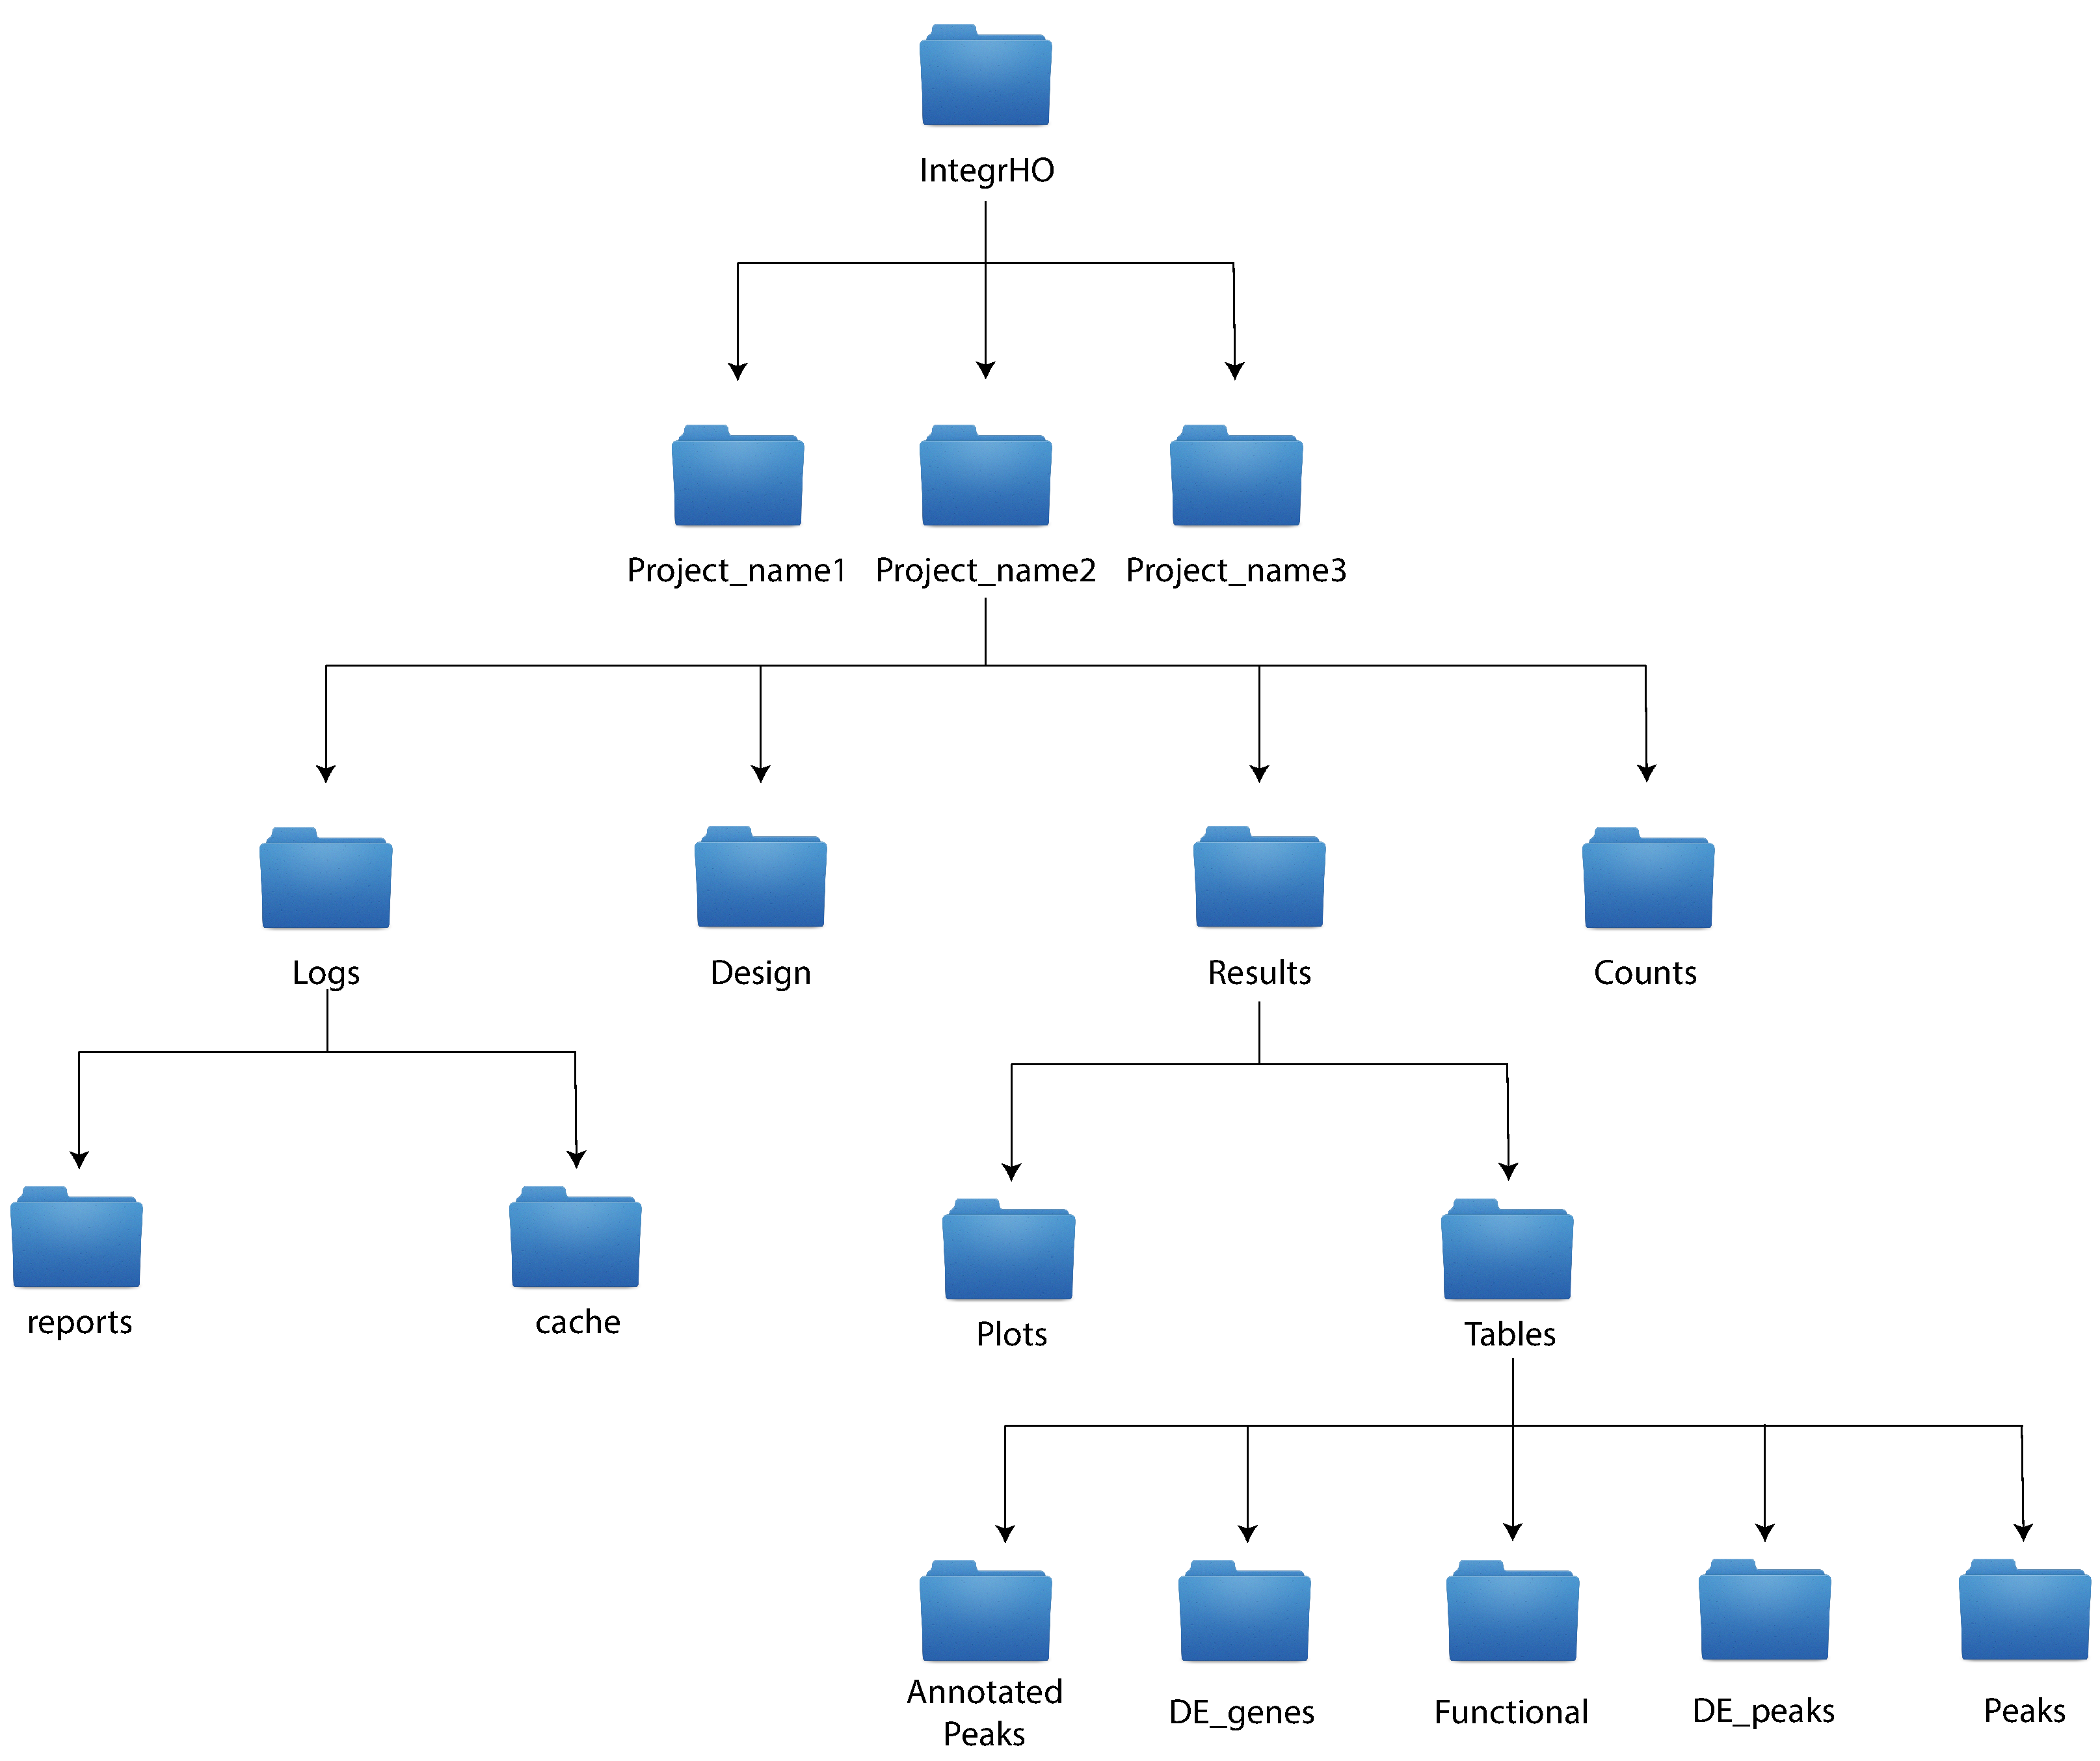
\includegraphics[width=\textwidth, keepaspectratio]{img/integrho/project_folder.pdf}
\caption[\gls{igro} folder tree]{A schematical representation of \gls{igro} project folder tree.}
\label{fig:integrhotree}
\end{figure}

In particular, we designed a \lstinline!R6ProjectClass!, which stores all the paths represented inside the figure \ref{fig:integrhotree}.
This allows fast access to the files stored in each folder, that will be processed specifically for each selected interface.


\subsection{Available Methodologies}

Unlike tools as Galaxy \cite{Hillman-Jackson2012} and Taverna \cite{Wolstencroft2013}, focused on analysis workflows, \gls{igro} gives to the user high freedom of interaction, reporting all performed steps in a human-readable \gls{html} report.
 
Actually, \gls{igro} methodologies have been organized in a way that the user can analyze every single omics, and afterwards, combine the results to obtain an integrated view of them.

In particular, we defined specific interfaces for \gls{rnaseq}, \gls{chipseq} and \gls{atacseq} data, providing additional interfaces for their integration, such as \textit{functional enrichment} and \textit{gene-peak} annotations.

Moreover, through the \lstinline!graphics! interface the user have the possibility to between a great variability of graphics, useful to explore data and results, both in pre-processing and post-processing phase, such as \textit{barplots}, \textit{correlation plots}, \textit{heatmap}, \textit{scatterplots}, \textit{keggmap}, etc.

Inside \gls{igro}, we take from granted that every omics data type is already mapped on a reference genome, with already available \gls{bam} files for every sample the user wants to investigate.

Figure \ref{fig:integrhopackscheme} shows a schematic representation of implemented packages inside \gls{igro}.
The upper part shows the single-omics packages used for the analysis of \gls{rnaseq}, \gls{chipseq} and \gls{atacseq}, while the lower part refers to the multi-omics integration, showing the packages used for \textit{functional analysis} and \textit{peak-gene annotations}.

\begin{figure}[ht]
\centering
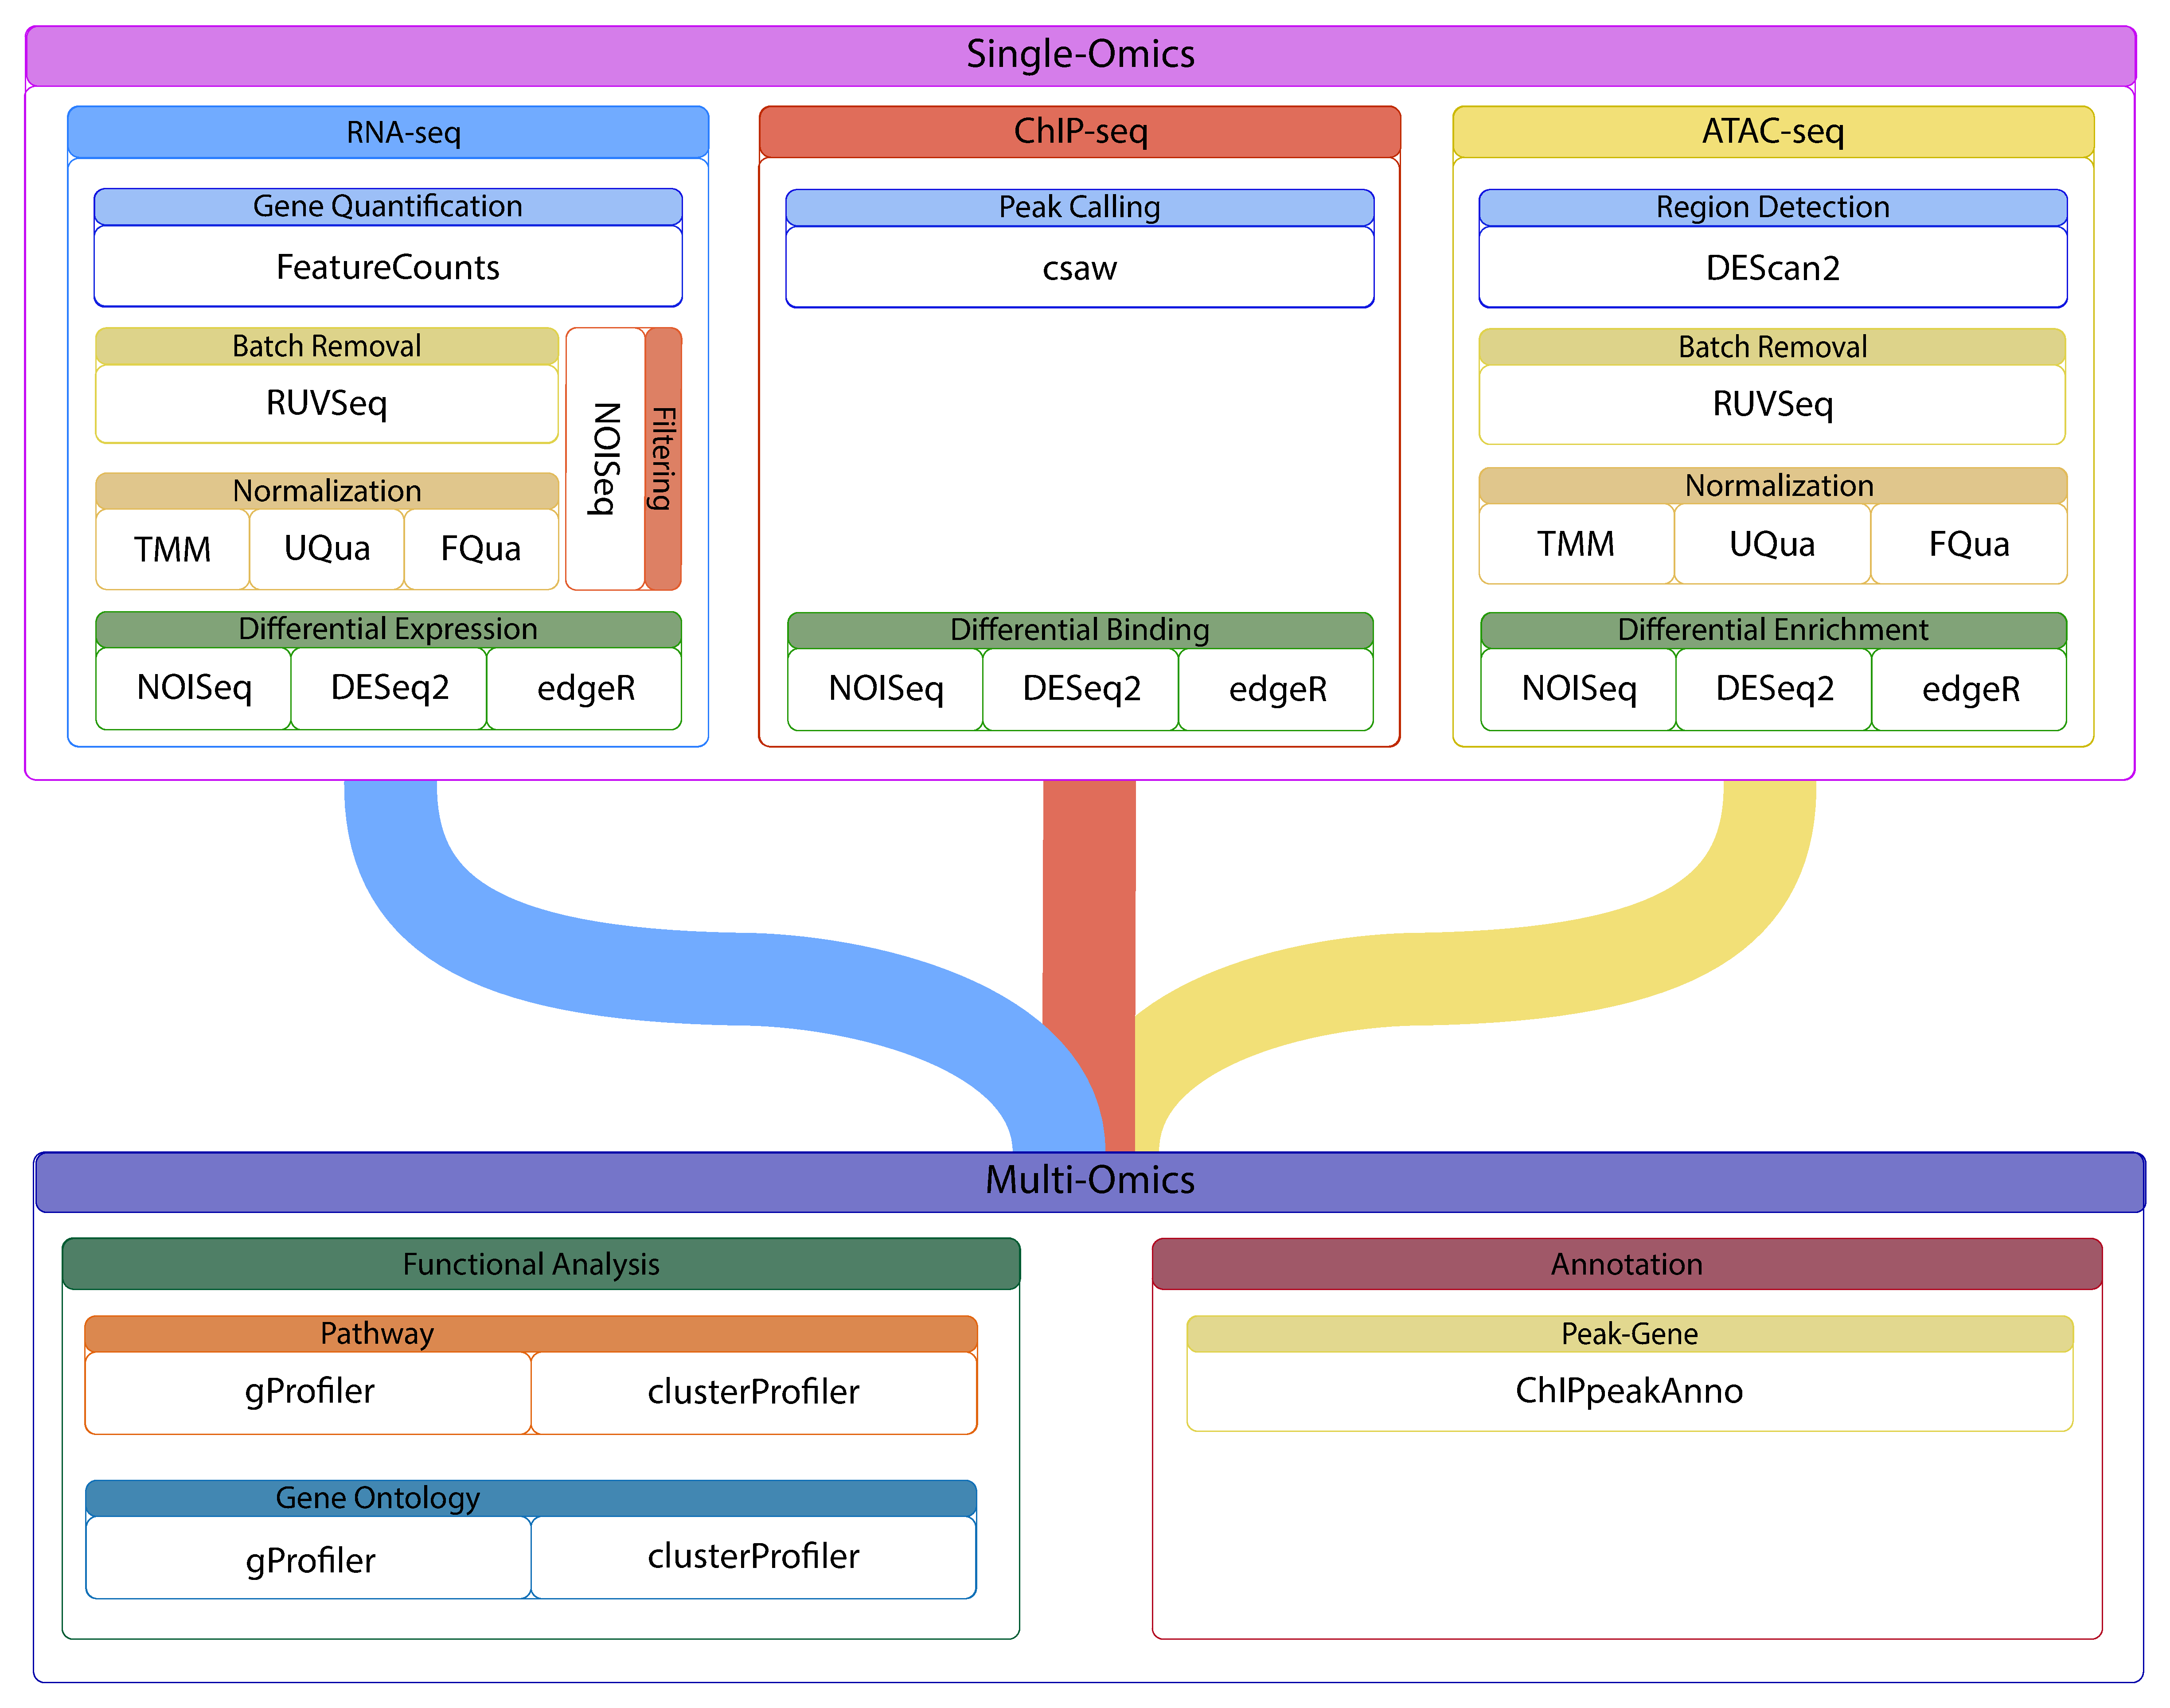
\includegraphics[width=\textwidth, keepaspectratio]{img/integrho/integrho_pack_scheme.pdf}
\caption[\gls{igro} packages scheme]{A schematical representation of packages included inside \gls{igro} web-platform.
The upper part shows the packages for the the single-omics analysis, while the lower part shows the packages for the multi-omics analysis.}
\label{fig:integrhopackscheme}
\end{figure}

%It implements not only the methodologies reported inside \textit{ticorser} for \gls{rnaseq} and \textit{DEScan2} for \gls{atacseq}, but implements also methodologies for \gls{chipseq} data analysis, complementing these aspects by providing functionalities for their integration at different levels, such as functional enrichment with Gene Ontology and Pathways and peaks-genes annotation.

\subsubsection{\gls{rnaseq}} \label{sec:integrhorna}
For \gls{rnaseq} we chose multiples methods for allowing the user to obtain a good overview of this omics analysis, focusing on \textit{Differential Expression} aspect.
In such a way, the user have several methodologies for accounting for a complete \gls{rnaseq} pipeline (refer to \ref{sec:rnaseq} section for a typical \gls{rnaseq} pipeline description).


%{\setlength{\parindent}{0cm}\textbf{Features Quantification}}

When working with \gls{rnaseq} data it is really important to quantify the reads contained inside the \gls{bam} files associating them to genomic features.
To do that, it is necessary a file with the genomic features description, typically a \gls{gtf} file (defined in \ref{sec:ticorseresults} section) describing the genomic coordinates for each feature (genes, transcripts etc.).

To account for genomic feature quantification, the user has to select the \lstinline!Quantify Counts! interface, designed for \lstinline!featureCounts! of \lstinline!Rsubread! R/Bioconductor package function \cite{Liao2014} appears.
The  \gls{bam} file paths for the \gls{rnaseq} data are automatically selected from the design matrix loaded during the project creation phase.

We choose proper widgets for selecting the reference genome and its annotation, it is also possible to configure the \lstinline!featureType! to use, while the \lstinline!attributeType! is set by default to \lstinline!gene_id!.
Additionally, parameters can be selected for \lstinline!allowMultiOverlap! and to select if the reads are \lstinline!paired!.
Finally, the number of threads to use can be set from 1 to 8.

At the end of the processing, the resulting count matrix is presented in the main part of the interface as a \lstinline!data.table! format, and automatically stored inside the \lstinline!IntegrHO/project_name/counts! folder.


%{\setlength{\parindent}{0cm}\textbf{Counts Filtering and Normalization}}

When working with \gls{rnaseq} data, several features are too low expressed to be kept, because their expression will affect the further analysis, leading to biased results.
When selecting the \lstinline!Filter Counts! the designed interface automatically loads the counts files inside the \lstinline!IntegrHO/project_name/counts!, otherwise allowing, with a \lstinline!fileInput! widget, to chose another count matrix file.
It is possible to switch between three different filtering methods (\textit{Proportion Test}, \textit{Wilcoxon Test}, \textit{CPM}), as defined inside the \lstinline!filtered.data! function of \textit{NOISeq} R/Bioconductor package \cite{Tarazona2011, Tarazona2015}.

The filtered-in features need to be normalized in order to be compared across multiple conditions.
Also in this case, a not proper data normalization can head to misleading results.

The same type of interface built for the filtering step is loaded when the \lstinline!Normalize Counts! menu voice is selected.
Three different normalization methods can be selected, the \textit{Trimmed Mean of M-values} \cite{Robinson2010}, the \textit{Upper Quartile} and the \textit{Full Quantile}.

Additionally, a main aspect of \gls{rnaseq} data analysis is to account for ''unwanted factors'' (batch effects) that, very often, affect the data.
This noises are part of the data because reflecting batch, library preparation, and other nuisance effects.

When selecting the \lstinline!Batch Effect! section there will be the possibility to apply the \textit{RUVs} or \textit{RUVg} methods from \textit{RUVSeq} R/Bioconductor package \cite{Risso2014h}.
Moreover, when selecting one of this methods, an additional file can be loaded, in order to upload an optional list of negative control genes.

To graphically inspect the normalized data two different plots will be presented into the main interface, the \gls{pca} and the \textit{boxplots} for before and after normalization of the samples.
This comparison is dictated by the need of inspecting the effects of noise removal from the data.

Finally, at the end of execution the filtered/normalized features, as \gls{tsv} file format, are stored inside the \lstinline!IntegrHO/project_name/counts! folder, adding at the end of the file name the ''transformation'' applied.


%{\setlength{\parindent}{0cm}\textbf{Differential Expression Methods}}

Finally, when the data are well normalized, the user can address for differential expression inspection of the samples.

In order to detect \glspl{deg}, we designed the \lstinline!Differential Expression Simple Design!, where it is possible to choose between four different methods.

The available count matrix files are automatically loaded from the \lstinline!IntegrHO/project_name/counts! folder.
Otherwise, the user can additionally load another count matrix file using the apposite file selector.

In order to address for the factors to analyze, the interface automatically gives the possibility to select the design matrix column name where to find them.
Additionally, two \lstinline!selectInput! widgets appear where to select the two factors to contrast.

We selected four different methods implemented inside \textit{edgeR}, \textit{DESeq2}, \textit{NOISeq} and \textit{NOISeqBio} R/Bioconductor packages \cite{Robinson2009, Love2014,Tarazona2012}.

In case of \textit{edgeR} we decided to use the \textit{Quasi-Likelihood} method for the differential expression.
While when using \textit{DESeq2} for this specific case we choose the \textit{Wald} test, as the authors suggest.
The \textit{NOISeq} package offers the possibility to discriminate between \textit{biological} and \textit{technical} replicates, computing a posterior probability in both cases, but applying different hypothesis tests.

The dedicated interface automatically shows a \lstinline!tabsetPanel! of 3 different tabs, within, respectively, a \textit{VolcanoPlot}, an \textit{MA-Plot} and the table of the \gls{deg} results.


\subsubsection{\gls{chipseq}} \label{sec:integrhochip}
\gls{chipseq} is a very common technique to investigate multiple epigenetic factors, the sequencing technique by itself identifies chromatin regions where specific proteins bind on.
Considering to have multiple \gls{bam} samples of \gls{chipseq} data, we constructed specific interfaces for peak calling and \glspl{dbs} detection.
Also in this case, we are focusing on the problem of detecting how the signal differs between multiple biological conditions.
We refer to \glspl{dbs} because of the nature of the biological data, coming it from proteins binding specific regions of the chromatin.

%{\setlength{\parindent}{0cm}\textbf{Peak Calling}}

Assuming that the samples are in \gls{bam} format, we assume that the user needs to reconstruct the signal of the chromatin regions binded by the interested protein.
We underline that a \gls{chipseq} experiment is ''protein specific'', because it involves using an antibody that is specific for a known protein.

For the \textbf{peak calling}, because of the lack of specific methods starting from \gls{bam} files in R, we implemented a dedicated interface for \textit{csaw} \cite{Lun2015} peak caller, which allows quantification for both broad and narrow peaks, typically resulting from \gls{hm} and \gls{tf} \gls{chipseq} data.

Firstly, it is possible to select the design matrix (stored inside \lstinline!IntegrHO/project_name/design! folder) and the column specifying the experiment.
In such a way, \gls{igro} is able to pick up the \gls{bam} filenames associated to the \gls{chipseq} experiments by itself.

Afterwards, the interface enables the specification of several parameters useful for the \lstinline!windowCounts! method of \textit{csaw} R/Bioconductor package.
The method constructs a count matrix where the rows indicate the detected windows of length \lstinline!window width! and the columns indicate samples.

Additional parameters selected for the analysis with the \textit{csaw} method are the \lstinline!paired end reads!, a flag for ignoring duplicated reads with \lstinline!ignore duplicates!, and the possibility to make the analysis only on a list of chromosomes, using the \lstinline!chromosomes list! implemented with a \lstinline!selectizeInput!.
The possibility to make parallel computing is implemented with the \lstinline!core number! widget (from 1 to 8).

At the end of the processing, the count matrix is shown into the main part of the interface, and it is saved as \gls{tsv} format, into the \lstinline!IntegrHO/project_name/results/tables/peaks! folder.
In order to distinguish the produced output from others, the results file is saved by adding the method name at the end of the filename.

%{\setlength{\parindent}{0cm}\textbf{Differential Binding}}
Once constructed a count matrix of genomic windows (features) on the rows and samples on the columns, in order to detect \glspl{dbs} across the conditions, we are able to apply the same methodologies designed for \gls{rnaseq} data (see section \ref{sec:integrhorna} for further details).
For this reason, we used the same methods as defined for \gls{rnaseq}, showing the results table as output.

Other methodologies for differential binding have been developed in R, such as the package \textit{DiffBind} \cite{Ross-Innes2012}, but at the moment we didn't implemented them yet.

Moreover, it is relevant for \gls{chipseq} data analysis to account for the ''right normalization'' to use.
The count matrix form allows to apply the same normalization methodologies developed for \gls{rnaseq} data, but at the moment we didn't implemented this aspect.
Additionally, it is still an open issue to study for the ''correctness'' of applied normalization on \gls{chipseq} data, even if some approaches have already been presented \cite{Angelini2015}.


\subsubsection{\gls{atacseq}} \label{sec:integrhoatac}

\gls{atacseq} is a sequencing technology for investigating chromatin accessible regions, which are typically associated on the identification of the instrumental epigenetic changes responsible for differential gene expression, cell proliferation, functional diversification and disease development (see \ref{sec:atacseq} for further details).

Thanks to the work made with \gls{descan} (chapter \ref{sec:descan2cap}), we had the possibility to deeply investigate \gls{atacseq} data, presenting a specific analysis workflow.
We tried to give access to the same methodologies, defined for \gls{descan}, herein \gls{igro}, in order to simplify and spread the proposed work.
%{\setlength{\parindent}{0cm}\textbf{Region Detection}}

As for the \gls{chipseq}, the user needs to reconstruct the signal across the entire genome by detecting the genomic regions.
%It needs to have already mapped the experimental sequences on a reference genome, producing \gls{bam} files for each of the samples under investigation.

In particular, to account for the regions detection, we built a specific interface for the peak caller defined in \gls{descan} (see section \ref{sec:descan2peakcall}).

As for the \textit{csaw}, the user can select the design matrix (stored inside \lstinline!IntegrHO/project_name/design! folder) and the column associated with the experiment definition.
Additional parameter selection is required for the selection of the \lstinline!genome name!, the \lstinline!bin size! for the genome binning, and for the \lstinline!max window! and \lstinline!min window! lengths.
Also, in this case, we gave the possibility to select for a multi-core computation with the \lstinline!core number! sliderInput widget.

The user can also select the \lstinline!peak score! threshold for filtering out the regions with a lower score than the threshold, and the \lstinline!samples threshold! for the alignment phase (see section \ref{sec:descan2filtering}).

In order to better compare \gls{descan} results with similar methods, such as \textit{casw}, we preferred to include also the \gls{descan} filtering method inside the \textit{region detection} interface.
In such a way, the presented output is a count matrix of detected regions (peaks) on the rows and samples on the columns.

After the reconstruction of the signal, it is a good norm to normalize the data, in order to remove unwanted factors biasing the data leading to misleading results.
Also in this case, we took advantages of the count matrix form to apply the same methodologies developed for \gls{rnaseq}, and doing the same for the detection of \glspl{der} (section \ref{sec:integrhorna}).

\subsubsection{Integration} \label{sec:integrhointegration}
The previously studied omics, even if not so many, already give the possibility to construct an integrated view of multiple cellular aspects.

For example, if we are able to collect samples of \gls{chipseq} for an \gls{hm} involved into the chromatin accessibility, and \gls{atacseq} samples with \gls{rnaseq} samples, we already are able to understand which regions of the genome are influenced by that  specific \gls{hm}, obtaining a crossed inspection with resulting region of \gls{atacseq}.
Moreover, we can look at how the gene expression has been influenced by these chromatin accession mechanisms.

To account even for simple integration problems like this one, we implemented functionalities for the \textbf{peak-gene annotation} of \glspl{der}/\glspl{dbs} with \glspl{deg} using \textit{ChIPpeakAnno}.

The interface allows for the selection of a \lstinline!peaks! file (\gls{der}/\gls{dbs}), automatically loaded from  \lstinline!IntegrHO/project_name/results/tables/peaks!.
Additionally, an \lstinline!annotation file! is required to retrieve the genomic features to annotate the peaks.
In alternative, a list of \glspl{deg} can be selected.
Other relevant parameters, such as the gene \lstinline!feature!  or the \lstinline!max distance! between the peaks and the genes, are needed for the right working of \lstinline!annotatePeakInBatch! function, defined inside the \lstinline!ChIPpeakAnno! R/Bioconductor package.

When the results are computed by the server side, they are showed with two plots organized in two panels of a \lstinline!tabsetPanel! widget. 
A \textit{pie chart} showing the percentage of detected features organized on their distance, and a table of annotated regions with corresponding genes.

Finally, a \gls{tsv} file, within annotated peaks, is saved inside the  \lstinline!IntegrHO/project_name/results/tables/annotated_peaks! folder, while the volcano plot, in \gls{html} format, is saved into the \lstinline!IntegrHO/project_name/results/plot! folder.

Another kind of integration is given by \textbf{functional annotation} analysis, where list of genes (annotated or resulting from differential experession analysis) can be used to detect cellular functional behaviours, thanks to databases born to annotate multiple gene contributing to specific cellular mechanisms (called pathways or gene ontology terms).

In order to interrogate these databases, several methodologies for functional analysis born \cite{Subramanian2005, Sales2012a, Reimand2016, Yu2012, Huang2009}.
The underlying idea of them is to use a list of genes to see which of them mostly \textit{up-regulate}/\textit{down-regulate} annotated cellular functional mechanisms

To account for this integration aspect we developed one interface for allowing the user to choose between two methods \textit{gProfiler} \cite{Reimand2016} and \textit{clusterProfiler} \cite{Yu2012}.
Both methodologies allow to investigate multiple databases, for pathways \textit{KEGG} and \textit{REACTOME}, while for Gene Ontology we give the possibility to choose between \gls{gobp}, \gls{gomf} and \gls{gocc}.

The interface automatically loads the file inside the \lstinline!IntegrHO/project_name/results/tables/annotated_peaks! and \lstinline!IntegrHO/project_name/results/tables/DE_genes! folders, giving the possibility to select the number corresponding to the column within the gene list.

In order to choose the method to apply, a \lstinline!selectInput! shiny widget gives the possibility to choose between the \textit{clusterProfiler} and the \textit{gProfiler} methods.
Moreover, the user has to select the type of functional annotation to do (pathway or Gene Ontology) and the database to use.

At the end of computations, \gls{igro} will present the table of the results in the main interface and will store them into the  \lstinline!IntegrHO/project_name/results/tables/functional! folder.

